\documentclass[11pt,a4paper]{article}

\usepackage[T1]{fontenc}
\usepackage[utf8]{inputenc}
\usepackage{mathpazo}
\usepackage[margin=2.6cm]{geometry}
\usepackage{amsmath}
\usepackage{booktabs}
\usepackage{longtable}
\usepackage{array}
\usepackage{graphicx}
\usepackage{caption}
\usepackage{microtype}
\usepackage[hidelinks]{hyperref}

\captionsetup{labelfont=bf, labelsep=period, font=small}
\captionsetup[table]{position=top, skip=4pt}
\setlength{\parskip}{0pt}

%  Le figure stanno nelle cartelle di output degli script: il paper non ne
%  tiene copie.
\graphicspath{{../studi/grafici_regime/}{../studi/grafici_ciclo/}{../studi/grafici_costruzione/}}

\newcommand{\figura}[3]{%
  \begin{figure}[htbp]\centering
  \includegraphics[width=#3\linewidth]{#1}
  \caption{#2}
  \end{figure}}

\title{\textbf{Market Regimes, Sector Rotation\\and Portfolio Construction in the S\&P 500, 2005--2026}}
\author{Giovanni Ferrante}
\date{November 2026}

\begin{document}
\maketitle

\begin{abstract}
\noindent
This paper asks whether market regimes can guide the allocation among the sectors of the S\&P 500, and how much the construction method matters once the stocks have been selected. The analysis uses the historical constituents of the index between February 2005 and June 2026, in a point-in-time backtest free of survivorship and look-ahead bias. Three regime definitions are compared: a hidden Markov model on market returns, a business-cycle indicator built from the macroeconomic data as they were published at each date, and the monetary-policy stance. Each regime conditions the choice of three among ten sectors, with the expected return of every sector in every regime learnt only from past data. None improves on a rotation that ignores the regime: the differences range from $-0.93\%$ to $-0.15\%$ a year, with no $t$-statistic above one in absolute value, and no rotation beats the index net of costs. The business-cycle regime does separate calm from turbulent markets, but sector prices move ahead of the real-time data. Holding the selected stocks fixed, six construction methods produce no significant difference in return, while volatility ranges from 13.9\% for minimum variance to 19.0\% for equal weighting, and every reduction is statistically significant.
\end{abstract}

\section{Introduction}

Sector rotation rests on a simple idea: sectors respond differently to the state of the economy and of markets, so an investor who recognises the state should hold the sectors that tend to do well in it. The idea is easy to state and hard to test. The state has to be identified with information available at the time, and the returns associated with each state have to be learnt from past data alone; otherwise the backtest rewards knowledge that no investor had.

This paper tests the idea on the historical constituents of the S\&P 500, around two questions. The first is whether a market regime, identified only with information available at each date, improves the allocation among sectors. Three regime definitions are compared:
\begin{itemize}
\item \textbf{statistical}: a hidden Markov model on market returns;
\item \textbf{economic}: business-cycle phases from real-time macroeconomic vintages;
\item \textbf{monetary policy}: the direction of the last move of the Federal Reserve.
\end{itemize}
The second question holds the selected stocks fixed and asks how much six weighting rules change return and risk.

Five principles guide the analysis.
\begin{itemize}
\item \textbf{Point-in-time universe.} Index membership is rebuilt month by month, so that removed stocks stay in the sample and their terminal returns are accounted for.
\item \textbf{No look-ahead.} Every quantity used at the formation date is computed with information available at that date, including the macroeconomic data, which are taken in the version that was published at the time.
\item \textbf{Costs from the start.} Costs are charged on traded weight from the first rebalancing, and both gross and net results are reported.
\item \textbf{Same sample.} All strategies are compared over the same months, with Newey--West standard errors.
\item \textbf{Specification fixed in advance.} Regime definitions must pass acceptance criteria fixed before any strategy return is computed, robustness checks verify rather than select, and every methodological decision is recorded with its motivation (Appendix~\ref{app:log}).
\end{itemize}

Section~\ref{sec:data} describes the data and Section~\ref{sec:rule} the rotation rule and the evaluation design. Section~\ref{sec:regimes} defines the three regimes and Section~\ref{sec:res2} reports the rotation results. Section~\ref{sec:res3} compares construction methods on a fixed selection. Sections~\ref{sec:lim} and~\ref{sec:concl} discuss the limitations and conclude.

\section{Data}\label{sec:data}

\subsection{Index membership and identifiers}

Market data are taken from LSEG Workspace. Index membership is rebuilt from two exports for the S\&P 500: the list of current constituents and the record of joiners and leavers. The reconstruction runs forward from the first date covered by the database, at the end of December 1994. Pairs of a leaver and a joiner for the same code on the same day are artefacts of corporate actions and are neutralised. Membership is stored as intervals that include the entry date and exclude the exit date.

Securities are identified by a stable key made of the organisation PermID and the share class, never by ticker or ISIN, so that a change of code does not interrupt a security's history. The crosswalk maps 1,025 instrument codes to 1,019 securities. Where several codes point to the same organisation, their monthly price series are compared before deciding whether they are the same security or distinct share classes.

\subsection{Panel, eligibility and exits}

The monthly panel contains total returns, prices and market capitalisations from January 2003 to June 2026, with one row per security and month: 204,574 observations on 1,016 securities. The full price history of each security is kept, whether or not it was in the index. Membership decides only which stocks are \emph{eligible} at a formation date. The index has between 493 and 507 members a month, with a median of 501. Missing returns are never replaced by zero.

A stock eligible at formation that has no return in the following month is almost always a corporate exit. In the backtest sample there are 51 permanent exits. For 18 of them the terminal value was reconstructed by documentary research from the cash and share terms of the transaction. The others receive a conservative terminal return of zero, equivalent to liquidation at the last known price. Two further exits fall in 2003--2004, a period used only to estimate sector returns, and are treated in the same way. Missing returns at the end of the sample are treated as censoring and shorten the sample instead.

\subsection{Benchmark, risk-free rate and factors}

The benchmark is the S\&P 500 Total Return index. The risk-free rate and the factors come from the Kenneth French data library, which also provides the monthly return of the whole US market from July 1926, used to estimate the statistical regime. As a check on the panel, a capitalisation-weighted index rebuilt from the reconstructed membership has a monthly correlation of 0.9989 with the official index, an annual return of 11.35\% against 11.11\% and a tracking error of 0.70\%.

\subsection{Sectors}

Sectors follow the TRBC economic classification. The GICS classification could not be used because LSEG returns no GICS sector for 290 of the 369 delisted instruments, whether as a current value or as of a historical date. Excluding them would have biased the sector baskets towards surviving firms. The TRBC classification covers every instrument; one sector with only three instruments is merged into Consumer Cyclicals, which leaves ten sectors.

\subsection{Macroeconomic and monetary data}

The macroeconomic series come from the Real-Time Data Set for Macroeconomists of the Federal Reserve Bank of Philadelphia (Croushore and Stark, 2001), which contains every monthly vintage of industrial production since November 1962 and of non-farm payrolls since December 1964. Ready-made activity indicators were considered and rejected because their vintages do not cover the sample: those of the Chicago Fed National Activity Index start in 2011 and those of the OECD leading indicator in 2018. The decisions of the Federal Open Market Committee on the federal funds target, 110 since 1990, are taken from the Federal Reserve Board and are never revised.

\section{Rotation rule and evaluation design}\label{sec:rule}

\paragraph{Sector baskets.} At each formation date the ten sectors are formed as capitalisation-weighted baskets of the index members. Their returns in the following month include the delisting returns described in Section~\ref{sec:data}.

\paragraph{Expected returns by regime.} Let $\pi_{\tau,k}$ be the probability of regime $k$ known at date $\tau$, and $r_{s,\tau+1}$ the return of sector $s$ in the following month. The expected return of sector $s$ in regime $k$, estimated at date $t$, is
\begin{equation}
\mu_{s,k}(t) = \frac{\sum_{\tau+1 \le t} \pi_{\tau,k}\, r_{s,\tau+1} + P\, m_s}{\sum_{\tau+1 \le t} \pi_{\tau,k} + P},
\end{equation}
where $m_s$ is the unconditional mean of the sector over the same window. The term $P$, set to 12 months, shrinks the estimate for a regime that has been observed only a few times. The forecast for $t+1$ mixes the regime estimates with the regime probabilities known at $t$, $\mathrm{E}_t[r_{s,t+1}] = \sum_k \pi_{t,k}\,\mu_{s,k}(t)$. Every quantity uses the regime \emph{as it was known} at each past date, never one recomputed later. The choice of sectors in each regime is therefore learnt from the data, not imposed from the literature.

\paragraph{Portfolio.} The three sectors with the highest forecast are held in equal proportions and capitalisation-weighted within each sector. Information up to the end of month $t$ forms the portfolio and the return is earned in month $t+1$. Rebalancing is monthly, and costs are 10 basis points per side on the traded weight, measured against the weights after a month of price drift. Turnover is reported as half the traded weight, so that 100\% corresponds to a complete renewal of the portfolio.

\paragraph{Comparisons.} The key comparison is with an \emph{unconditional rotation}, which applies the same rule with a single regime and so ranks sectors by their historical mean. The difference between a regime rotation and the unconditional rotation isolates the contribution of the regime. Equally weighted sectors and the index complete the comparison.

\paragraph{Evaluation.} All strategies are evaluated over the same 257 months, from February 2005 to June 2026; sector returns from 2003 serve only as the initial estimation window. Returns and volatilities are annualised, and the Sharpe ratio uses the mean and standard deviation of monthly excess returns over the one-month T-bill. Mean differences between strategies are tested with Newey--West standard errors (Newey and West, 1987). Robustness checks change one element at a time from the base case.

\section{Three definitions of the market regime}\label{sec:regimes}

\subsection{A statistical regime: hidden Markov model}

The first regime is a two-state Gaussian hidden Markov model (Hamilton, 1989) on the monthly market excess return from July 1926.
\begin{itemize}
\item \textbf{Estimation.} The model is re-estimated by maximum likelihood at every formation date on an expanding window.
\item \textbf{Probabilities.} Only filtered probabilities are used; the forecast for $t+1$ is the filtered probability at $t$ multiplied by the transition matrix.
\item \textbf{Labels.} The states are ordered by volatility, so that the labels do not switch between estimates.
\end{itemize}
At the last date the calm state has a mean of 12.8\% and a volatility of 12.9\% a year, and the turbulent state a mean of $-16.3\%$ and a volatility of 34.9\%; the two persist for about 50 and 9 months on average. Two rules from the literature serve as comparisons: the market trading above its 10-month moving average (Faber, 2007), and a positive market return over the previous 24 months (Daniel and Moskowitz, 2016).

\figura{figure_R1_regime_probability.png}{Real-time probability of the adverse regime for the hidden Markov model and the two rules}{0.88}

\subsection{An economic regime: the business cycle in real time}

The second regime measures the business cycle with industrial production and non-farm payrolls. At each date $t$ only the vintage published in month $t$ is used, whose last observation is month $t-1$; in 279 of 281 dates the lag is exactly one month and it never falls to zero.

\paragraph{Indicator.} Within that vintage, the 12-month growth of each series is measured relative to its own 10-year moving average and standardised. The two series are averaged, and the average is smoothed over three months, in the manner of the three-month average of the Chicago Fed National Activity Index. A moving average is preferred to a two-sided filter of the Hodrick--Prescott type, whose estimates at the end of the sample are unreliable in real time (Orphanides and van Norden, 2002; Hamilton, 2018).

\paragraph{Acceptance criteria.} Before the regime was used in any strategy, three criteria were fixed and evaluated on the phases alone:
\begin{itemize}
\item each phase covers at least 10\% of the months;
\item each phase lasts at least five months on average, the minimum phase length of Bry and Boschan (1971);
\item the NBER recessions fall in the weakest phase.
\end{itemize}

\paragraph{Revisions.} The first specification, with four phases (level $\times$ direction), the mean since 1948 as the reference and no smoothing, failed the criteria: 47\% of months were classified as contraction and the phase changed 81 times. The specification was revised three times, in an order agreed in advance and before any strategy return had been computed:
\begin{enumerate}
\item a 10-year moving average as the reference, and the smoothed indicator;
\item a new phase adopted only after five consecutive months of confirmation;
\item two phases instead of four.
\end{enumerate}
Each revision is recorded in Appendix~\ref{app:log}.

\paragraph{Final regime.} It has two phases, above and below trend. It classifies 22\% of months as below trend, changes phase four times after 2005 and places all 20 NBER recession months below trend. The four-phase version, whose recovery phase covers only 8.2\% of months, is kept as a robustness check.

\subsection{A policy regime: the monetary-policy stance}

The third regime follows Conover, Jensen, Johnson and Mercer (2008). Policy is \emph{expansionary} after a cut in the federal funds target and \emph{restrictive} after a hike, until a move in the opposite direction. The decision counts if it was announced by the end of month $t$. At the zero lower bound no move occurs and the regime remains expansionary, consistent with the policy actually pursued.

\figura{figure_C1_regimes.png}{Business-cycle and monetary-policy regimes known at each formation date; grey bands are NBER recessions, shown for reference only}{0.95}

\section{Results: regimes and sector rotation}\label{sec:res2}

Table~\ref{tab:rotperf} gives the central result: \textbf{no regime improves sector rotation}.

\begin{itemize}
\item \textbf{Unconditional rotation.} It earns 9.02\% a year net of costs, below both the equally weighted sectors (10.48\%) and the index (11.11\%).
\item \textbf{Hidden Markov model.} $-0.19\%$ a year relative to the unconditional rotation ($t=-0.30$).
\item \textbf{Business cycle.} $-0.93\%$ ($t=-0.91$).
\item \textbf{Monetary policy.} $-0.15\%$ ($t=-0.10$).
\item \textbf{Moving-average rule.} The only difference with a $t$-statistic above one in absolute value is negative, at $-1.92\%$, and significant only at 10\%. It is driven by turnover, which more than doubles.
\end{itemize}

\begin{table}[htbp]
\centering
\small
\caption{Sector rotation with and without regime signals, net of costs}\label{tab:rotperf}
\setbox0\hbox{%
\begin{tabular}{lrrrrrrr}
\toprule
Strategy & Return & Volatility & Sharpe & Max drawdown & Turnover & vs unconditional & t-stat \\
\midrule
\multicolumn{8}{l}{\textit{No regime}} \\
Equal-weight sectors & 10.48\% & 14.70\% & 0.64 & $-$50.49\% & 1.75\% & -- & -- \\
Unconditional rotation & 9.02\% & 17.01\% & 0.50 & $-$50.71\% & 7.29\% & -- & -- \\
\addlinespace
\multicolumn{8}{l}{\textit{Statistical and rule-based regimes}} \\
HMM regime rotation & 8.85\% & 16.84\% & 0.49 & $-$51.03\% & 10.08\% & $-$0.19\% & $-$0.30 \\
SMA regime rotation & 7.07\% & 16.45\% & 0.40 & $-$50.52\% & 15.39\% & $-$1.92\%$^{*}$ & $-$1.72 \\
Trend regime rotation & 10.03\% & 16.82\% & 0.56 & $-$47.84\% & 10.16\% & 0.89\% & 0.72 \\
\addlinespace
\multicolumn{8}{l}{\textit{Economic regimes}} \\
Business-cycle rotation & 8.20\% & 15.99\% & 0.47 & $-$52.88\% & 12.20\% & $-$0.93\% & $-$0.91 \\
Monetary-policy rotation & 8.99\% & 16.31\% & 0.51 & $-$53.08\% & 11.52\% & $-$0.15\% & $-$0.10 \\
\addlinespace
\multicolumn{8}{l}{\textit{Index}} \\
Benchmark (S\&P 500 TR) & 11.11\% & 14.90\% & 0.67 & $-$50.95\% & -- & -- & -- \\
\bottomrule
\end{tabular}}%
\ifdim\wd0>\linewidth\resizebox{\linewidth}{!}{\box0}\else\box0\fi
\par\vspace{3pt}
\parbox{0.95\linewidth}{\footnotesize Three TRBC economic sectors held, equally weighted, cap-weighted within each sector; monthly rebalancing; 10 bp per side. The last two columns report the mean annualised difference from the unconditional rotation and its Newey-West t-statistic.}
\end{table}


\figura{figure_C2_wealth.png}{Growth of 100 invested in the rotation strategies and the index, net of costs (log scale)}{0.9}

Table~\ref{tab:rotdiag} shows why the three regimes fail for different reasons.

\paragraph{Hidden Markov model.} It identifies volatility, not economic weakness. In the month after a turbulent signal the market was more volatile (24.5\% against 14.3\%) but earned \emph{more} (20.2\% against 11.1\%), because turbulent spells in this sample ended in rebounds.

\paragraph{Business cycle.} It does separate market conditions: after a below-trend month the market earned 6.7\% with a volatility of 22.1\%, against 13.4\% and 12.9\% above trend. Its failure lies elsewhere, as Figure~\ref{fig:fasi} shows. In below-trend phases, the sectors with the highest returns in the following month were the cyclical ones (Basic Materials, Consumer Cyclicals and Technology), not the defensive ones. Prices anticipate the recovery before the real-time data record it, consistent with evidence that industry returns lead the economy (Hong, Torous and Valkanov, 2007). With only three below-trend episodes in the sample, the estimates of sector returns by phase also rest on very few observations. In the 2007 slowdown, for example, the rotation bought cyclical sectors ahead of the 2008 crash.

\paragraph{Monetary policy.} It barely separates the market at all: 11.5\% after expansionary and 12.4\% after restrictive months.

\begin{table}[htbp]
\centering
\small
\caption{Regimes in the backtest sample and the market in the following month}\label{tab:rotdiag}
\setbox0\hbox{%
\begin{tabular}{lrrrr}
\toprule
Regime & Share & Switches & Market return & Market volatility \\
\midrule
\multicolumn{5}{l}{\textit{HMM (2 states)}} \\
Favourable & 91.8\% & 10 & 11.13\% & 14.33\% \\
Adverse & 8.2\% & 10 & 20.18\% & 24.46\% \\
\addlinespace
\multicolumn{5}{l}{\textit{10-month moving average}} \\
Favourable & 80.2\% & 30 & 12.03\% & 11.70\% \\
Adverse & 19.8\% & 30 & 11.23\% & 25.41\% \\
\addlinespace
\multicolumn{5}{l}{\textit{24-month market return}} \\
Favourable & 87.5\% & 10 & 11.08\% & 13.64\% \\
Adverse & 12.5\% & 10 & 17.45\% & 24.50\% \\
\addlinespace
\multicolumn{5}{l}{\textit{Business cycle}} \\
Above trend & 77.8\% & 4 & 13.35\% & 12.86\% \\
Below trend & 22.2\% & 4 & 6.70\% & 22.07\% \\
\addlinespace
\multicolumn{5}{l}{\textit{Monetary policy}} \\
Expansionary & 58.8\% & 5 & 11.48\% & 16.70\% \\
Restrictive & 41.2\% & 5 & 12.43\% & 13.28\% \\
\bottomrule
\end{tabular}}%
\ifdim\wd0>\linewidth\resizebox{\linewidth}{!}{\box0}\else\box0\fi
\par\vspace{3pt}
\parbox{0.95\linewidth}{\footnotesize Share of the 257 formation months in each regime, number of regime switches, and annualised mean and volatility of the market return (Kenneth French) in the month after the regime is observed. Descriptive only: no strategy uses these figures.}
\end{table}


\begin{figure}[htbp]\centering
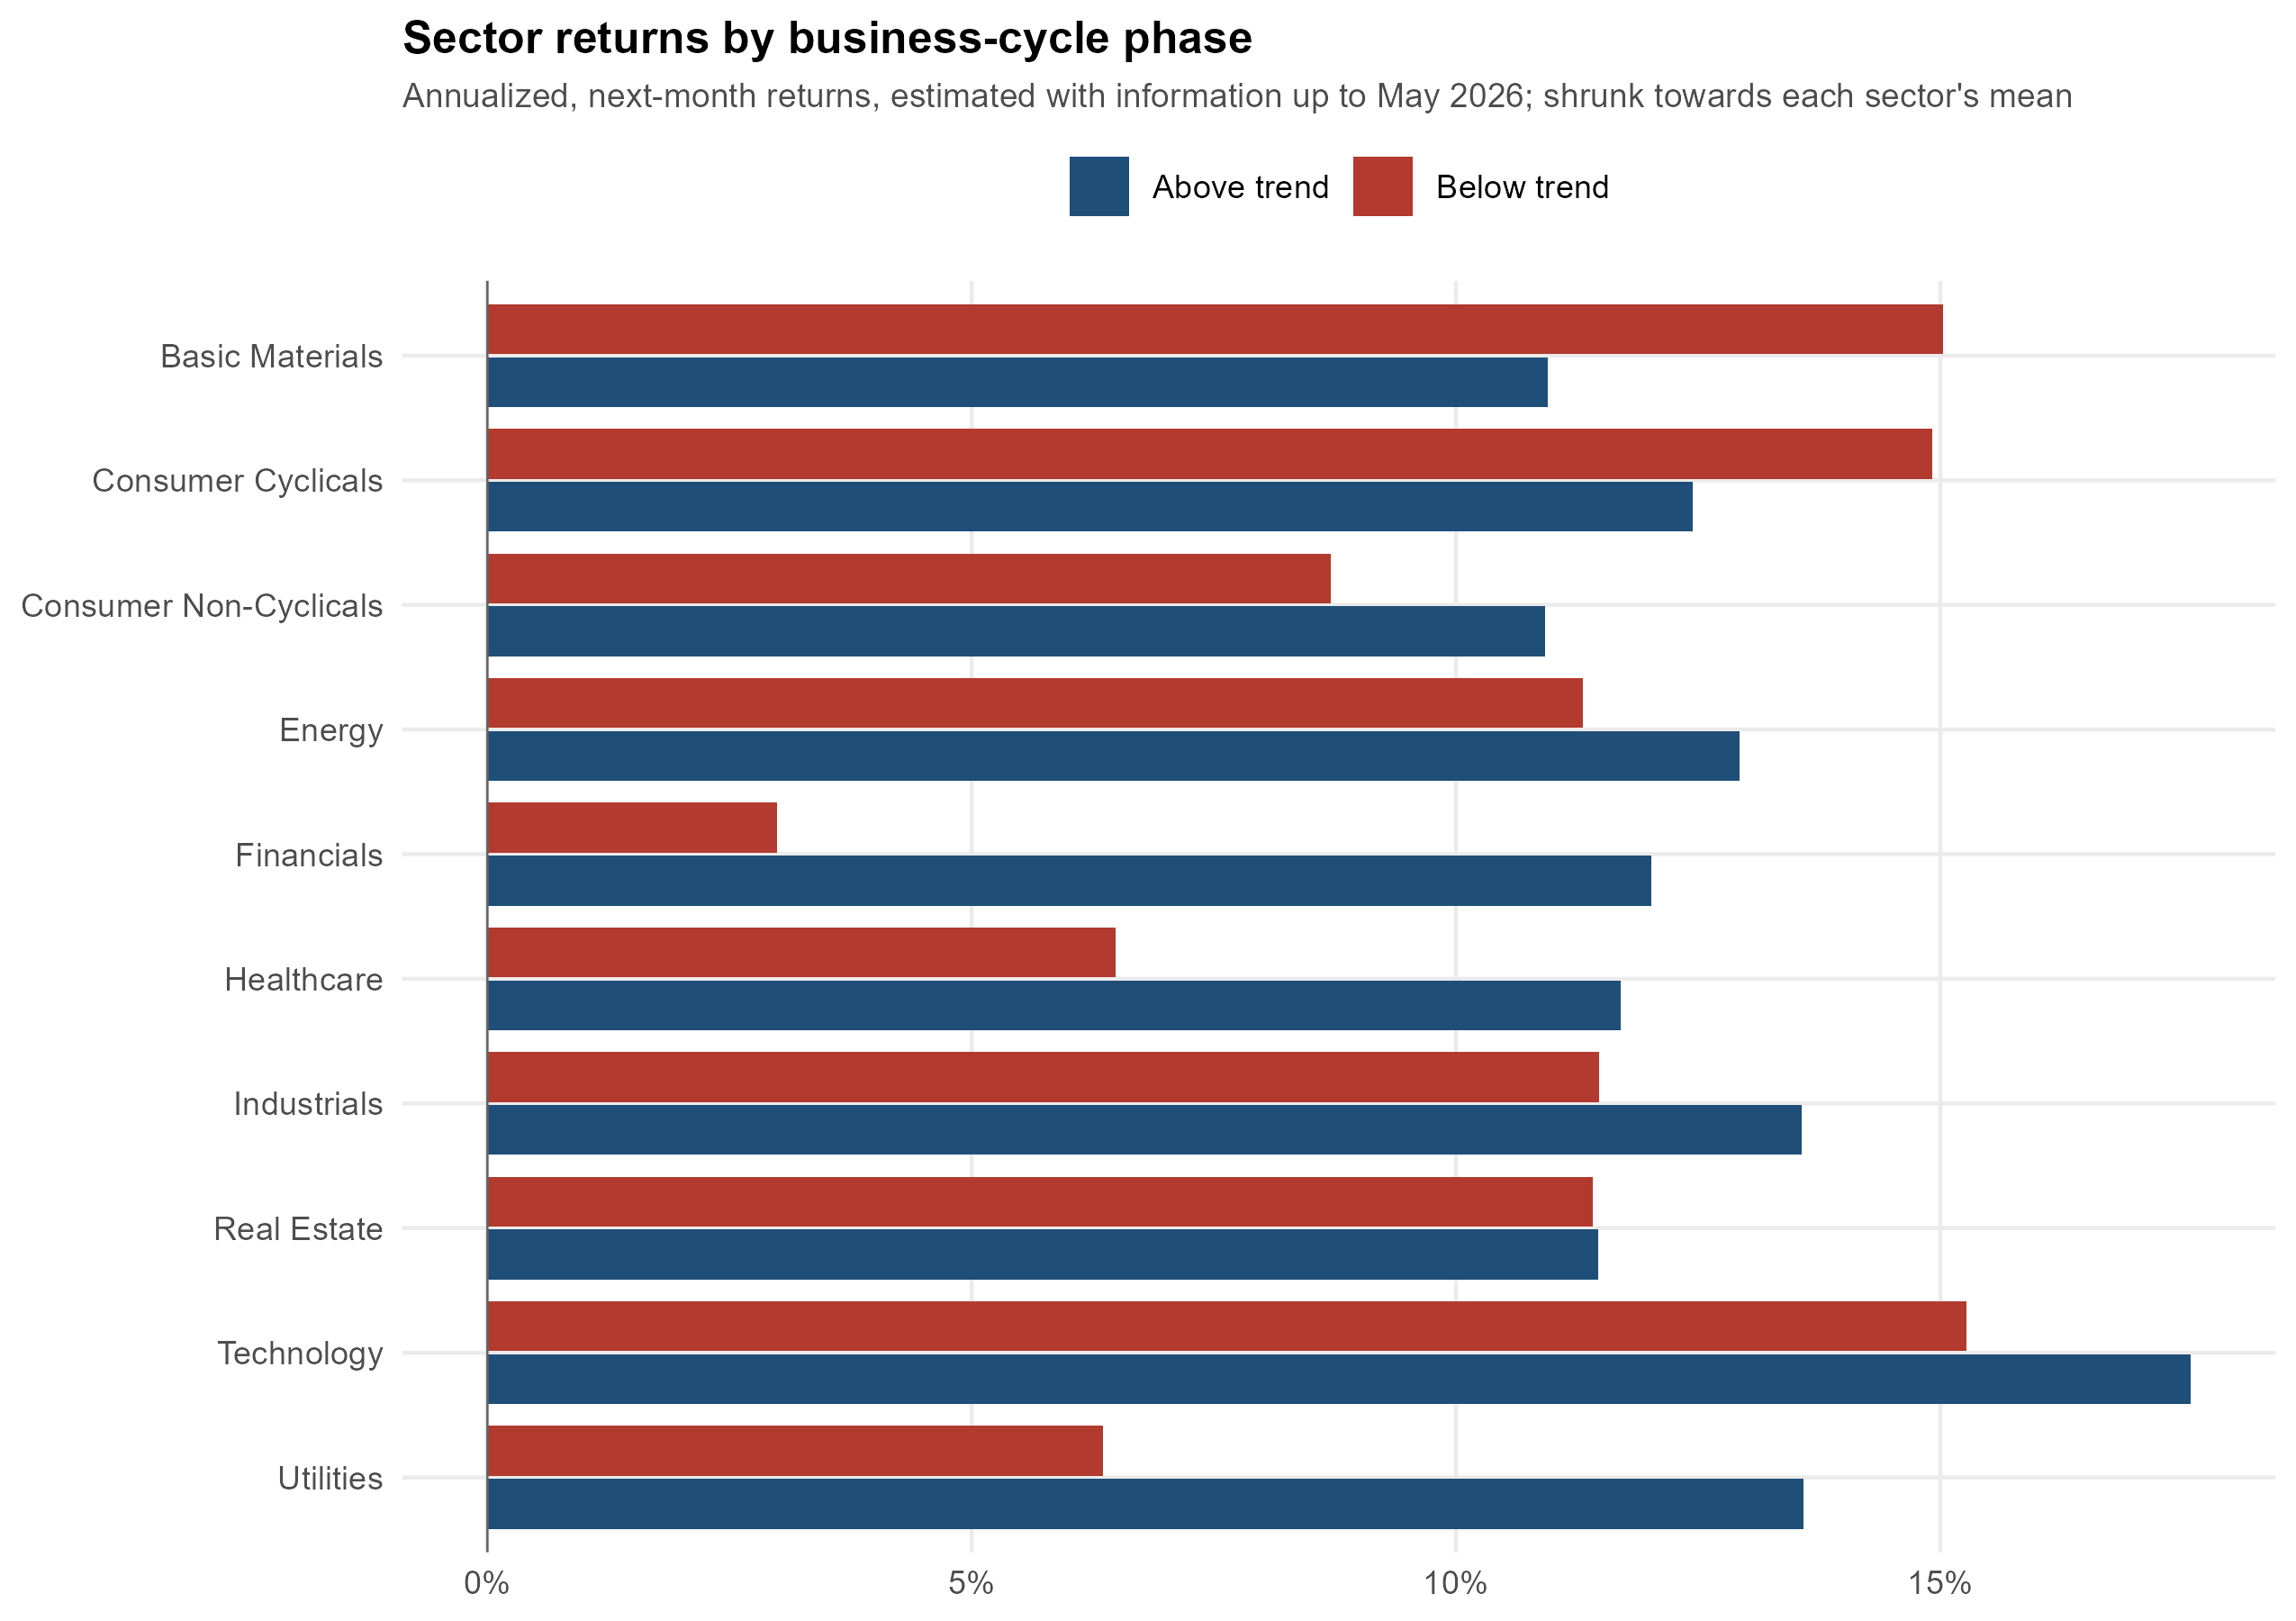
\includegraphics[width=0.78\linewidth]{figure_C4_returns_by_phase.png}
\caption{Sector returns in the month after each business-cycle phase, as estimated at the last formation date}\label{fig:fasi}
\end{figure}

Table~\ref{tab:rotrob} varies the business-cycle rotation one element at a time. None of the nine variants improves significantly on the unconditional rotation. The most favourable, the four-phase version, adds 0.89\% a year with a $t$-statistic of 0.68.

\begin{table}[htbp]
\centering
\small
\caption{Robustness of the business-cycle rotation, net of costs}\label{tab:rotrob}
\setbox0\hbox{%
\begin{tabular}{lrrrrr}
\toprule
Variant & Return & Sharpe & Turnover & vs unconditional & t-stat \\
\midrule
\multicolumn{6}{l}{\textit{Baseline}} \\
Baseline & 8.20\% & 0.47 & 12.20\% & $-$0.93\% & $-$0.91 \\
\addlinespace
\multicolumn{6}{l}{\textit{Cycle phases}} \\
4 phases (level x direction) & 10.30\% & 0.61 & 13.61\% & 0.89\% & 0.68 \\
No confirmation & 8.42\% & 0.48 & 12.35\% & $-$0.73\% & $-$0.77 \\
\addlinespace
\multicolumn{6}{l}{\textit{Cycle indicator}} \\
Industrial production only & 8.17\% & 0.46 & 12.61\% & $-$0.90\% & $-$0.83 \\
Payroll employment only & 7.97\% & 0.45 & 14.15\% & $-$1.14\% & $-$0.98 \\
\addlinespace
\multicolumn{6}{l}{\textit{Sectors held}} \\
Top 2 sectors & 8.73\% & 0.48 & 13.68\% & $-$0.30\% & $-$0.29 \\
Top 4 sectors & 9.64\% & 0.57 & 9.40\% & 0.27\% & 0.26 \\
\addlinespace
\multicolumn{6}{l}{\textit{Shrinkage}} \\
Prior 36 months & 8.44\% & 0.48 & 11.31\% & $-$0.66\% & $-$0.79 \\
\addlinespace
\multicolumn{6}{l}{\textit{Transaction costs}} \\
25 bp & 7.72\% & 0.44 & 12.20\% & $-$1.37\% & $-$1.32 \\
50 bp & 6.93\% & 0.39 & 12.20\% & $-$2.10\% & $-$1.97 \\
\bottomrule
\end{tabular}}%
\ifdim\wd0>\linewidth\resizebox{\linewidth}{!}{\box0}\else\box0\fi
\par\vspace{3pt}
\parbox{0.95\linewidth}{\footnotesize Baseline: two phases (above or below trend), industrial production and payrolls, five-month confirmation, three sectors held. Each variant changes one element.}
\end{table}


\section{Results: construction methods on a fixed selection}\label{sec:res3}

The rotation decides which stocks are held, not how much of each. This section holds the selection fixed and changes only the weighting.

\paragraph{Selection.} At each date, the candidate stocks are the members of the three sectors chosen by the business-cycle rotation.

\paragraph{Methods.} Six methods weight them:
\begin{itemize}
\item the construction used so far (sectors equally weighted, capitalisation weights within each);
\item equal weighting;
\item capitalisation weighting;
\item inverse volatility;
\item equal risk contribution (Maillard, Roncalli and Teïletche, 2010);
\item long-only minimum variance.
\end{itemize}

\paragraph{Risk model and common set.} Covariances are estimated on up to 60 months of past returns with the shrinkage estimator of Ledoit and Wolf (2004), with a median shrinkage intensity of 0.18. Inverse volatility uses sample volatilities, because shrinkage towards a common variance would flatten its weights. To ensure that every method weights the same stocks, only candidates with a complete return history in the estimation window are used. This excludes a median of five of 125 candidates, or 1.7\% of their market value.

Table~\ref{tab:cosperf} shows that construction changes risk much more than return.

\begin{itemize}
\item \textbf{Return.} Net returns lie between 7.7\% and 8.1\% for every method except capitalisation weighting, at 10.65\%.
\item \textbf{Volatility.} It ranges from 19.0\% for equal weighting to 13.9\% for minimum variance.
\item \textbf{Minimum variance.} It also has the smallest drawdown ($-47.1\%$) and a beta of 0.70. The price is concentration (on average 28 stocks held, with an effective number of 16) and the highest turnover, 25\% a month against 11--16\% for the other methods. Its ex-ante volatility of 8.9\% understates the realised 13.9\%, the familiar in-sample optimism of optimised portfolios.
\end{itemize}

\begin{table}[htbp]
\centering
\footnotesize
\caption{Construction methods on the stocks selected by the business-cycle rotation, net of costs}\label{tab:cosperf}
\setbox0\hbox{%
\begin{tabular}{lrrrrrrrr}
\toprule
Method & Return & Volatility & Sharpe & Max drawdown & Turnover & Eff. stocks & Max weight & Beta \\
\midrule
Sectors EW, cap-weighted within & 7.90\% & 15.86\% & 0.45 & $-$52.78\% & 12.23\% & 42.8 & 8.3\% & 0.91 \\
Equal-weighted & 7.99\% & 19.01\% & 0.41 & $-$57.48\% & 14.91\% & 134.9 & 0.8\% & 1.12 \\
Cap-weighted & 10.65\% & 17.69\% & 0.57 & $-$51.64\% & 10.86\% & 25.5 & 14.0\% & 1.01 \\
Inverse volatility & 8.03\% & 17.50\% & 0.44 & $-$54.20\% & 15.72\% & 124.3 & 1.6\% & 1.03 \\
Equal risk contribution & 7.91\% & 16.91\% & 0.44 & $-$52.02\% & 16.46\% & 110.7 & 2.9\% & 1.00 \\
Minimum variance & 7.72\% & 13.90\% & 0.49 & $-$47.06\% & 25.27\% & 16.3 & 12.5\% & 0.70 \\
Benchmark (S\&P 500 TR) & 11.11\% & 14.90\% & 0.67 & $-$50.95\% & -- & -- & -- & -- \\
\bottomrule
\end{tabular}}%
\ifdim\wd0>\linewidth\resizebox{\linewidth}{!}{\box0}\else\box0\fi
\par\vspace{3pt}
\parbox{0.95\linewidth}{\footnotesize All methods weight the same stocks at each date (members of the three selected sectors with a complete 60-month return history). Effective number of stocks: inverse of the sum of squared weights, averaged over formation dates. Market beta from a market-model regression of net excess returns.}
\end{table}


Table~\ref{tab:cossig} turns these observations into tests. Against equal weighting, no return difference is significant: the largest, for capitalisation weighting, is 2.16\% a year with a $t$-statistic of 1.20. Every reduction in volatility, by contrast, is significant at 1\% under the Pitman--Morgan test for paired samples (Pitman, 1939; Morgan, 1939).

\begin{table}[htbp]
\centering
\small
\caption{Construction methods against equal weighting}\label{tab:cossig}
\setbox0\hbox{%
\begin{tabular}{lrrr}
\toprule
Comparison & Estimate & t-stat & p-value \\
\midrule
\multicolumn{4}{l}{\textit{Return difference versus equal-weighted}} \\
Sectors EW, cap-weighted within minus Equal-weighted & $-$0.67\% & $-$0.51 & 0.610 \\
Cap-weighted minus Equal-weighted & 2.16\% & 1.20 & 0.229 \\
Inverse volatility minus Equal-weighted & $-$0.25\% & $-$0.43 & 0.670 \\
Equal risk contribution minus Equal-weighted & $-$0.47\% & $-$0.59 & 0.558 \\
Minimum variance minus Equal-weighted & $-$1.14\% & $-$0.48 & 0.628 \\
\addlinespace
\multicolumn{4}{l}{\textit{Volatility versus equal-weighted (Pitman-Morgan), net}} \\
Sectors EW, cap-weighted within minus Equal-weighted & ratio 0.834$^{***}$ & $-$10.03 & 0.000 \\
Cap-weighted minus Equal-weighted & ratio 0.931$^{***}$ & $-$2.92 & 0.004 \\
Inverse volatility minus Equal-weighted & ratio 0.921$^{***}$ & $-$11.15 & 0.000 \\
Equal risk contribution minus Equal-weighted & ratio 0.890$^{***}$ & $-$12.46 & 0.000 \\
Minimum variance minus Equal-weighted & ratio 0.731$^{***}$ & $-$9.44 & 0.000 \\
\bottomrule
\end{tabular}}%
\ifdim\wd0>\linewidth\resizebox{\linewidth}{!}{\box0}\else\box0\fi
\par\vspace{3pt}
\parbox{0.95\linewidth}{\footnotesize Return differences: mean annualised difference with Newey-West t-statistics. Volatility: ratio of the volatility of each method to that of the equal-weighted portfolio, with the Pitman-Morgan test for paired samples.}
\end{table}


\figura{figure_K3_risk_return.png}{Risk and return of the construction methods and the index, net of costs}{0.72}

Table~\ref{tab:cosrob} shows that a cap of 5\% on individual weights leaves the conclusions unchanged. It also shows that restricting the sample to the common set of stocks costs the reference construction 0.3 percentage points a year.

\begin{table}[htbp]
\centering
\footnotesize
\caption{Construction methods: weight cap and common set of stocks, net of costs}\label{tab:cosrob}
\setbox0\hbox{%
\begin{tabular}{lrrrrr}
\toprule
Variant & Return & Volatility & Sharpe & Turnover & Eff. stocks \\
\midrule
\multicolumn{6}{l}{\textit{5\% weight cap}} \\
Cap-weighted, 5\% cap & 9.95\% & 17.99\% & 0.53 & 12.19\% & 47.2 \\
Equal risk contribution, 5\% cap & 7.91\% & 16.92\% & 0.44 & 16.44\% & 110.9 \\
Minimum variance, 5\% cap & 7.50\% & 14.07\% & 0.47 & 24.00\% & 25.0 \\
\addlinespace
\multicolumn{6}{l}{\textit{Common set}} \\
Previous study: all candidates (sectors EW, cap within) & 8.20\% & 15.99\% & 0.47 & 12.20\% & -- \\
This study: common set (sectors EW, cap within) & 7.90\% & 15.86\% & 0.45 & 12.23\% & 42.8 \\
\bottomrule
\end{tabular}}%
\ifdim\wd0>\linewidth\resizebox{\linewidth}{!}{\box0}\else\box0\fi
\end{table}


\section{Limitations}\label{sec:lim}

\begin{itemize}
\item \textbf{Sector classification.} The most recent TRBC sector of each security is applied to the whole sample, so reclassifications are projected backwards.
\item \textbf{Short sector history.} Sector returns start in 2003, and the business-cycle estimates rest on three below-trend episodes. A longer history, for example from industry portfolios before 2003, would make the regime-conditional estimates more reliable, but would require a mapping between classifications.
\item \textbf{Revisions of the regime specification.} The business-cycle regime was revised three times against criteria fixed in advance and applied to the phases alone. No rotation return had been computed at that point, but the process is documented in the decision log.
\item \textbf{Market series.} The hidden Markov model uses the French market series as a proxy for an investable index.
\item \textbf{Transaction costs.} They are a flat 10 basis points per side, without a market-impact component, which may understate the cost of the high-turnover strategies.
\item \textbf{Delisting returns.} Documentary terminal values are available for 18 of the 51 permanent exits; the others receive the conservative zero.
\item \textbf{Tests not performed.} Differences in Sharpe ratios between construction methods are not tested formally.
\end{itemize}

\section{Conclusion}\label{sec:concl}

Two results emerge from a common, point-in-time framework.

\begin{enumerate}
\item \textbf{Regimes and sector rotation.} Three independent regime definitions, statistical, economic and monetary, do not improve sector rotation among S\&P 500 constituents, and no rotation beats the index net of costs. The business-cycle regime carries real information about market risk, but sector prices move ahead of the real-time data on which it is built, and the sample offers too few cycles to learn which sectors to hold in each phase.
\item \textbf{Construction on a fixed selection.} With the stocks held fixed, construction methods produce large and significant differences in risk, but none in return.
\end{enumerate}

The common thread is that the regime and the weighting scheme are better suited to controlling risk than to generating return. Two extensions follow naturally. The first is to estimate the sector returns of each phase on a longer history, so that they rest on more business cycles. The second is to use the volatility regime of the hidden Markov model to scale the exposure to equities rather than to choose among sectors.

\appendix
\section{Decision log}\label{app:log}

Table~\ref{tab:log} lists the choices that affect the numbers and, where one was considered, the alternative that was not adopted. A full log with evidence and dates accompanies the code.

{\small
\begin{longtable}{>{\raggedright\arraybackslash}p{0.19\linewidth}>{\raggedright\arraybackslash}p{0.41\linewidth}>{\raggedright\arraybackslash}p{0.32\linewidth}}
\caption{Methodological decisions}\label{tab:log}\\
\toprule
Topic & Decision & Alternative considered \\
\midrule
\endfirsthead
\toprule
Topic & Decision & Alternative considered \\
\midrule
\endhead
\bottomrule
\endfoot
Universe & Point-in-time S\&P 500 members, membership rebuilt from joiner and leaver events & Current constituents (survivorship bias) \\
Identifiers & PermID and share class; multi-code groups checked on price series & Ticker or ISIN \\
Exits & Documentary terminal value where available, otherwise zero; exits in the 2003--2004 estimation window treated the same way & Exclusion of stocks without a next-month return \\
Benchmark & S\&P 500 Total Return; risk-free rate and factors from the French library & Price index \\
Costs & 10 bp per side on traded weight after drift & 25 and 50 bp (Table~\ref{tab:rotrob}) \\
Sector classification & TRBC economic sectors for all securities & GICS (missing for most delisted securities); GICS with TRBC mapped for delisted ones \\
Rotation rule & Regime-conditional means estimated from past data, shrinkage of 12 months, three sectors held & Cyclical and defensive sectors fixed in advance \\
Statistical regime & Two-state HMM on market excess returns since 1926, expanding window, filtered probabilities & Three states (robustness); S\&P 500 index history from LSEG \\
Choice of economic regimes & Business cycle as the main regime, monetary policy as comparison & Yield-curve and credit-spread regime; real-time recession indicator (too rare) \\
Macro data & Philadelphia Fed real-time vintages of industrial production and payrolls & CFNAI and OECD leading indicator, whose vintages start in 2011 and 2018 \\
Cycle indicator & 12-month growth relative to a 10-year moving average, three-month smoothing & Mean since 1948; Hodrick--Prescott trend \\
Cycle phases & Two phases with five-month confirmation, chosen against criteria fixed in advance & Four phases (robustness); machine-learning regime detection \\
Monetary regime & Direction of the last FOMC move on the federal funds target & Direction of the two-year Treasury yield \\
Construction comparison & Six methods on a common set of stocks, no weight cap & 5\% cap (Table~\ref{tab:cosrob}) \\
Risk model & Ledoit--Wolf covariance on up to 60 months; sample volatilities for inverse volatility & Sample covariance \\
Inference & Newey--West errors; Pitman--Morgan test for volatilities & Tests of Sharpe-ratio differences (not performed) \\
\end{longtable}
}

\section{Reproducibility}

The analysis is written in R.
\begin{itemize}
\item \textbf{Data pipeline.} A script built on generic modules for point-in-time data, backtesting and evaluation rebuilds the data layer: membership, crosswalk, monthly series, delisting returns, benchmark and factors.
\item \textbf{Studies.} Three scripts run the hidden Markov model, the business-cycle and monetary-policy regimes, and the construction comparison. Each one re-runs the parts of the pipeline it depends on.
\item \textbf{Outputs.} Tables are written to CSV files and Excel workbooks, figures to PNG files, and the tables of this paper are generated directly from the CSV files.
\item \textbf{Data.} The French, Philadelphia Fed and Federal Reserve inputs are public and downloaded by the scripts. The LSEG inputs are licensed, so the data are not part of the public repository, and the data layer can be rebuilt only with LSEG Workspace access.
\end{itemize}

\section*{References}
\begingroup
\small
\setlength{\parindent}{-1.5em}\setlength{\leftskip}{1.5em}\setlength{\parskip}{3pt}

Bry, G., and Boschan, C. (1971). \emph{Cyclical Analysis of Time Series: Selected Procedures and Computer Programs}. Technical Paper 20. National Bureau of Economic Research.

Conover, C. M., Jensen, G. R., Johnson, R. R., and Mercer, J. M. (2008). Sector rotation and monetary conditions. \emph{Journal of Investing}, 17(1), 34--46.

Croushore, D., and Stark, T. (2001). A real-time data set for macroeconomists. \emph{Journal of Econometrics}, 105(1), 111--130.

Daniel, K., and Moskowitz, T. J. (2016). Momentum crashes. \emph{Journal of Financial Economics}, 122(2), 221--247.

Faber, M. T. (2007). A quantitative approach to tactical asset allocation. \emph{Journal of Wealth Management}, 9(4), 69--79.

Hamilton, J. D. (1989). A new approach to the economic analysis of nonstationary time series and the business cycle. \emph{Econometrica}, 57(2), 357--384.

Hamilton, J. D. (2018). Why you should never use the Hodrick--Prescott filter. \emph{Review of Economics and Statistics}, 100(5), 831--843.

Hong, H., Torous, W., and Valkanov, R. (2007). Do industries lead stock markets? \emph{Journal of Financial Economics}, 83(2), 367--396.

Ledoit, O., and Wolf, M. (2004). A well-conditioned estimator for large-dimensional covariance matrices. \emph{Journal of Multivariate Analysis}, 88(2), 365--411.

Maillard, S., Roncalli, T., and Teïletche, J. (2010). The properties of equally weighted risk contribution portfolios. \emph{Journal of Portfolio Management}, 36(4), 60--70.

Morgan, W. A. (1939). A test for the significance of the difference between the two variances in a sample from a normal bivariate population. \emph{Biometrika}, 31(1/2), 13--19.

Newey, W. K., and West, K. D. (1987). A simple, positive semi-definite, heteroskedasticity and autocorrelation consistent covariance matrix. \emph{Econometrica}, 55(3), 703--708.

Orphanides, A., and van Norden, S. (2002). The unreliability of output-gap estimates in real time. \emph{Review of Economics and Statistics}, 84(4), 569--583.

Pitman, E. J. G. (1939). A note on normal correlation. \emph{Biometrika}, 31(1/2), 9--12.

\endgroup

\end{document}
